%!TEX TS-program = xelatex 
%!TEX encoding = UTF-8 Unicode 
%!TEX root = DESpecs.tex


% {quis}  --> {quod}


\section{File Conventions}
\label{section file conventions}

\begin{mainruleLessImportant}
Save the text in plain text format (§.txt§) with Unicode §utf-8§ encoding. If the text is saved in more than one file, number the parts, for example §Euclid_part_001.txt§, §Euclid_part_002.txt§, and so on. Create a §zip§ archive from all files.

We will also need the list of unknown characters (see \sect{section unknown characters}) for each file. It should have the same filename
as the text it is from, but with the postfix §-unknown§ (e.\,g.
§Euclid-unknown.pdf§) . If the list is handwritten, scan it and save it as PDF file.
\end{mainruleLessImportant}


\section{General Markup}

\tocspace
\subsection{Pages}

\begin{mainrule}
Type the entire contents of one page, then go on to the next page. Do not mix the contents of different pages.
\end{mainrule}

\subsubsection{Page Breaks, Page Numbers and Running Heads}
\label{section page breaks}

\begin{mainrule}
Page breaks are marked by §<pb>§. If the page has a page number, type it within the §<pb>§ tag, e.g. §<pb 6>§. Type the page number exactly as it appears in the book. If there is a running head on the page, it is marked by §<rh>§ and §</rh>§. Type the running head immediately after the §<pb>§ tag. 
\end{mainrule}

\begin{clarification}
Insert a blank line before each §<pb>§ tag. 
The position of the page number, e.g. at the top or bottom of the page, will not be encoded. Type the §<pb>§ and §<rh>§ tags before you type any content of the page. Do not type spaces within words. If there is a horizontal line below the running head, do not type it.
\end{clarification}

\begin{sampleImage}[ 1: \, arabic page number]{montag_mark_pagenumber_runninghead.jpg}
\begin{typeLatin}
\bold{<pb} 2\bold{><rh>}GEOMET. ELEMENT. EVCLIDIS\bold{</rh>} \\
$unt ӕquales. 16 Et hic quidem punctus, centrum circuli dicitur.\bold{</p>} \\
\untranscribedText
\end{typeLatin}
\end{sampleImage}

\begin{crossref}
For §$§ and §æ§ see \sect{section characters to be typed directly}. For ligatures, e.g. {\fontspec[Ligatures=Rare]{Hoefler Text} ct}, see \sect{section latin ligatures}. §</p>§ marks the end of a paragraph (\sect{section paragraphs}). For spaces before and after punctuation marks see \sect{section latin punctuation}.
\end{crossref}

\begin{note}
The §<p>§ for the beginning of the paragraph is on the previous page. 
\end{note}

\vspace{3mm}
\begin{sampleImage}[ 2: \, roman page number]{montag_roemische_seitenzahl} 
\begin{typeLatin}
\bold{<pb} vij\bold{><rh>_}PREFACE\bold{_}.\bold{</rh>}
\end{typeLatin}
\end{sampleImage}

\begin{crossref}
For §_ _§ see \sect{section italics}.
\end{crossref}


\subsubsection{Catchwords and Signatures}
\label{section catchwords and signatures}

\begin{mainrule}
Do not type catchwords or signatures.
\end{mainrule}

\begin{clarification}
In most cases, catchwords and signatures are at the bottom of the page.
\end{clarification}

\begin{sampleImage}{catchword_signature_neu}

\notTranscribed

The left rectangle contains the signature (§Ec 2§) and the right rectangle the catchword (§Volo§).
\end{sampleImage}


\tocspace
\subsection{Text Blocks}

\begin{mainrule}
Type a return after each line of the printed page.
\end{mainrule}

\begin{clarification}
Do not insert a space at the end of the line. 
\end{clarification}

\subsubsection{Headings}
\label{section headings}

\begin{mainrule}
Headings are marked by §<h>§ and §</h>§.
\end{mainrule}

\begin{clarification}
All headings are tagged in the same way, regardless of the font size. Do not type spaces within words. If the text is centered, this will not be encoded.
\end{clarification}

\begin{sampleImageSmall}{width=.7\linewidth}{montag_headings_euclid_233}
\begin{typeLatin}
\bold{<h>}EUCLIDIS \\
ELEMENTORUM \\
LIBER DECIMUS.\bold{</h>}
\end{typeLatin}
or alternatively, if you are unsure whether each line is a separate heading:
\begin{typeLatin}
\bold{<h>}EUCLIDIS\bold{</h>} \\
\bold{<h>}ELEMENTORUM\bold{</h>} \\
\bold{<h>}LIBER DECIMUS.\bold{</h>}
\end{typeLatin}
\end{sampleImageSmall}


\subsubsection{Paragraphs} 
\label{section paragraphs}

\begin{mainrule}
Paragraphs are marked by §<p>§ and §</p>§.
\end{mainrule}

\begin{clarification}
Make sure that for each §<p>§ there is a corresponding §</p>§ somewhere. If a paragraph starts and ends on different pages, the §<p>§ and §</p>§ tags are on these different pages.
If the first line of the paragraph is indented, this will not be encoded. If the text is centered, this will not be encoded either.
%A change in the font style, for example a line in italics, may indicate a new paragraph. TODO: Probably this rule will not apply very often. Leave it out? Put it somewhere else? (it occurs in the example in \sect{Structural markup general example})
\end{clarification}

\begin{sampleImage}{paragraph_benedetti_299}
\begin{typeLatin}
\untranscribedText \bold{</p>} \\
\bold{<p>}Secunda cau$a e$t, quia quoduis graue corpus, aut per naturam, aut per vim mo- \\
tum, rectitudinem itineris naturaliter appetat, quod clarè cogno$cere po$$umus, \\
proijciendo lapides funda, & circunducentes brachium, nam funes tanto maius \\
pondus acquirunt, & manum tanto magis onerant, quanto velocius voluitur funda, \\
& incitatur motus, quod ab appetitu naturali in$ito ei corpori per lineã rectam pro- \\
grediendi procedit. Vnde fit, vt pondus circunferentiæ ip$ius rotæ, tanto facilius cir- \\
cunuoluatur, & ex $eip$o tanto longiori tempore moueatur, quanto longius di$tat à \\
centro, cum eius iter tanto minus $it curuum. Hanc igitur ob cau$am, rota, quanto \\
maior erit, eiu$\bs´q; pondus tanto magis vicinum circunferentiæ, tanto magis durabit \\
impetus motus a$$umptus.\bold{</p>} \\
\bold{<p>} \untranscribedText
\end{typeLatin}
\end{sampleImage}

\begin{crossref}
For  §à§ and §ã§ see \sect{section characters to be typed directly}. For  §\´q§ see \sect{section other diacritics}. See also the example in \sect{Structural markup general example}.
\end{crossref}

\begin{note}
Headings (\sect{section headings}) are marked by §<h>§~§</h>§ instead of §<p>§~§</p>§. Block quotations  (\sect{section block quotations}) are marked by §<q>§~§</q>§ instead of §<p>§~§</p>§. The §<p>§ and §</p>§ tags should not be used in marginal notes (\sect{section marginal notes}) or footnotes (\sect{section footnotes}). 
\end{note}


\subsubsection{Block Quotations}
\label{section block quotations}

\begin{mainrule}
A block quotation is marked by §<q>§ and §</q>§. Do not type repeating quotation symbols.
\end{mainrule}

\begin{clarification}
The §<q>§ and §</q>§ replace the §<p>§ and §</p>§ tags.
\end{clarification}

\begin{sampleImage}{quotation_2.jpg} 
\begin{typeLatin}
\bold{<p>}Nec non vbi ita inquit.\bold{</p>}\\
\bold{<q>}Et $i (modo credimus) vnum\\
I$$e diem $ine Sole ferunt, incendia lumen\\
Præbebant.\bold{</q>}\\
\bold{<p>}Quod autem à Patre in$truatur etiam de cur$u annuali,\\
videbitur vbi ita dicit.\bold{</p>}\\
\bold{<q>}Nitor in aduer$um, nec me, qui cætera vincit.\\
Impetus, & rapido contrarius euehor orbi.\bold{</q>} \\
\bold{<p>}Et vbi ita loquitur.\bold{</p>}
\end{typeLatin}
\end{sampleImage}

\begin{note}
For inline quotations within a paragraph, type the quotation marks exactly as they appear in the text.
\end{note}


\subsubsection{Footers}

\begin{mainruleLessImportant}
If you can identify a paragraph as a footer, use §<h>§ and §</h>§ instead of §<p>§ and §</p>§.
\end{mainruleLessImportant}

\begin{crossref}
§<h>§ and §</h>§ is the tag for headings (\sect{section headings}).
\end{crossref}

\begin{sampleImage}{mkbsp_footer_benedetti.jpg}
\begin{typeLatin}
\bold{<p>} \someText \\
quem quidem tractatum cum quibu$dam alijs meis $peculationibus in lucem prode\\
re cupio, $i fieri poterit, antequam ad directionem mei Horo$copi cum corpore\\
Martis An\li{ae}ret\li{ae} perueniam, qu\li{ae} quidem directio circa annum mille$imum quin-\\
gente$imum nonage$imum $ecundum eueniet.\bold{</p>}\\
\bold{<h>}FINIS.\bold{</h>}
\end{typeLatin}

\end{sampleImage}

\begin{crossref}
For §{ae}§ see \sect{section latin ligatures}.
\end{crossref}


\tocspace
\subsection{Columns}
\label{section columns}

\begin{mainrule}
Columns are marked by §<col>§ and §</col>§. Assign a number to each column and type it in the §<col>§ tag.
\end{mainrule}

\begin{clarification}
Type the §<col>§ and §</col>§ tags on separate lines.
\end{clarification}

\mehrzeilen

\begin{mainruleLessImportant}

\begin{tabular}{@{}llll}
\htsc{Example 1: \, a real page} &&& \htsc{Example 2: \, how to type columns} \\
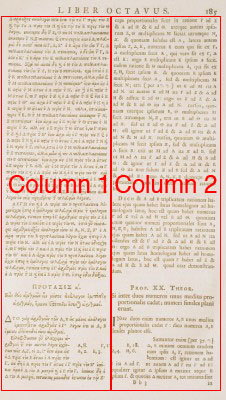
\includegraphics[scale=0.6]{wholepagecolumns2}  &&
\multicolumn{2}{l}{
\includegraphics[scale=0.63]{three_columns}} \\
\parbox[t]{4.5cm}{\small \vspace{1mm}
\notTranscribed \\[2mm]
Note that the page number and the running head are not part of a column.}
&&&
\parbox[t]{4cm}{ \vspace{-3mm}
\begin{typeLatin}
\bold{<col 1>} \\
\bold{<p>}This is one \\ column ...\bold{</p>} \\
\bold{</col>} \\ 
\bold{<col 2>} \\
\bold{<p>}This is \\ another \\ column.\bold{</p>} \\
\bold{</col>} \\ 
\bold{<col 3>} \\
\bold{<p>}And there \\ might be \\ yet another \\ column.\bold{</p>} \\
\bold{</col>} \\
\end{typeLatin}}
\end{tabular}

\end{mainruleLessImportant}

\begin{note}
If there is no running text in the columns, they may be not be separate columns, but a table (\sect{section tables}). If in doubt, check the example there.
\end{note}


\tocspace
\subsection{Tables}
\label{section tables}

\subsubsection{Nomenclature}
\label{section tables overview}

%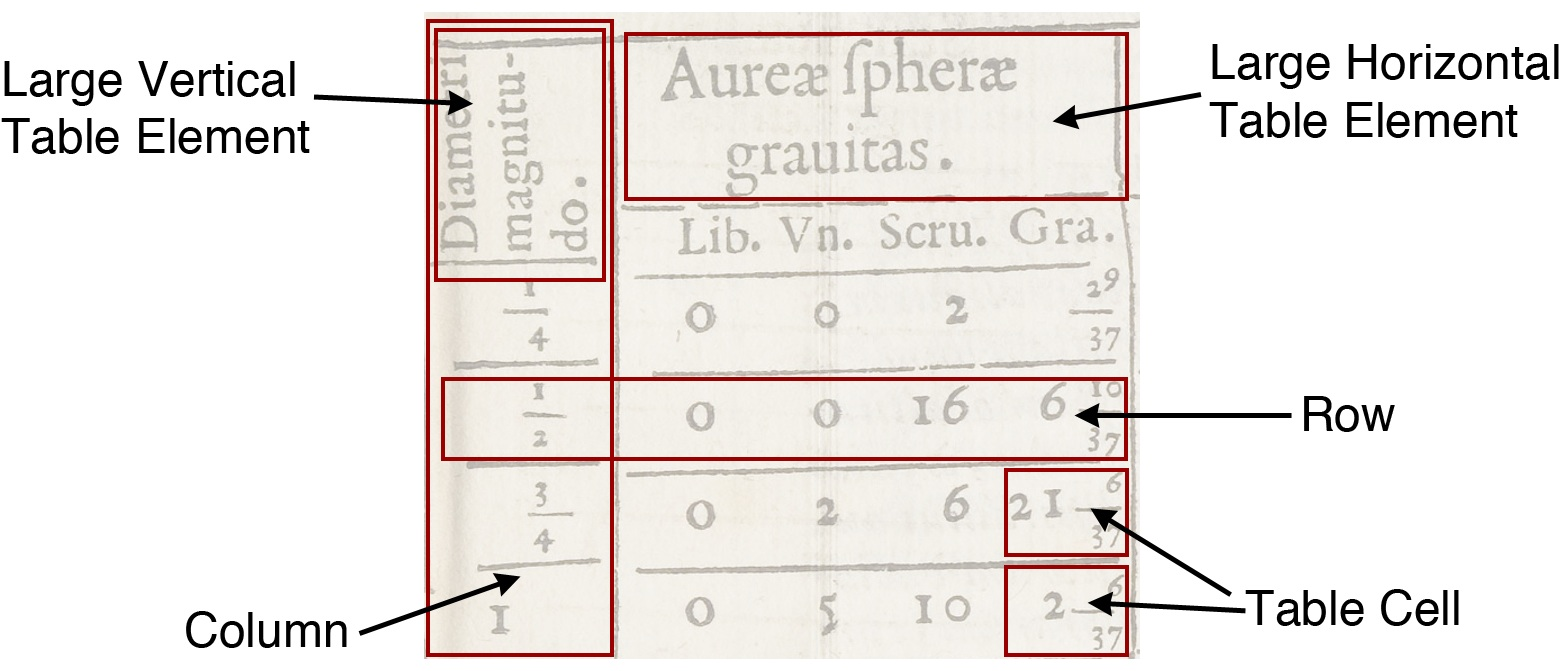
\includegraphics[width=14cm]{bettertable9}
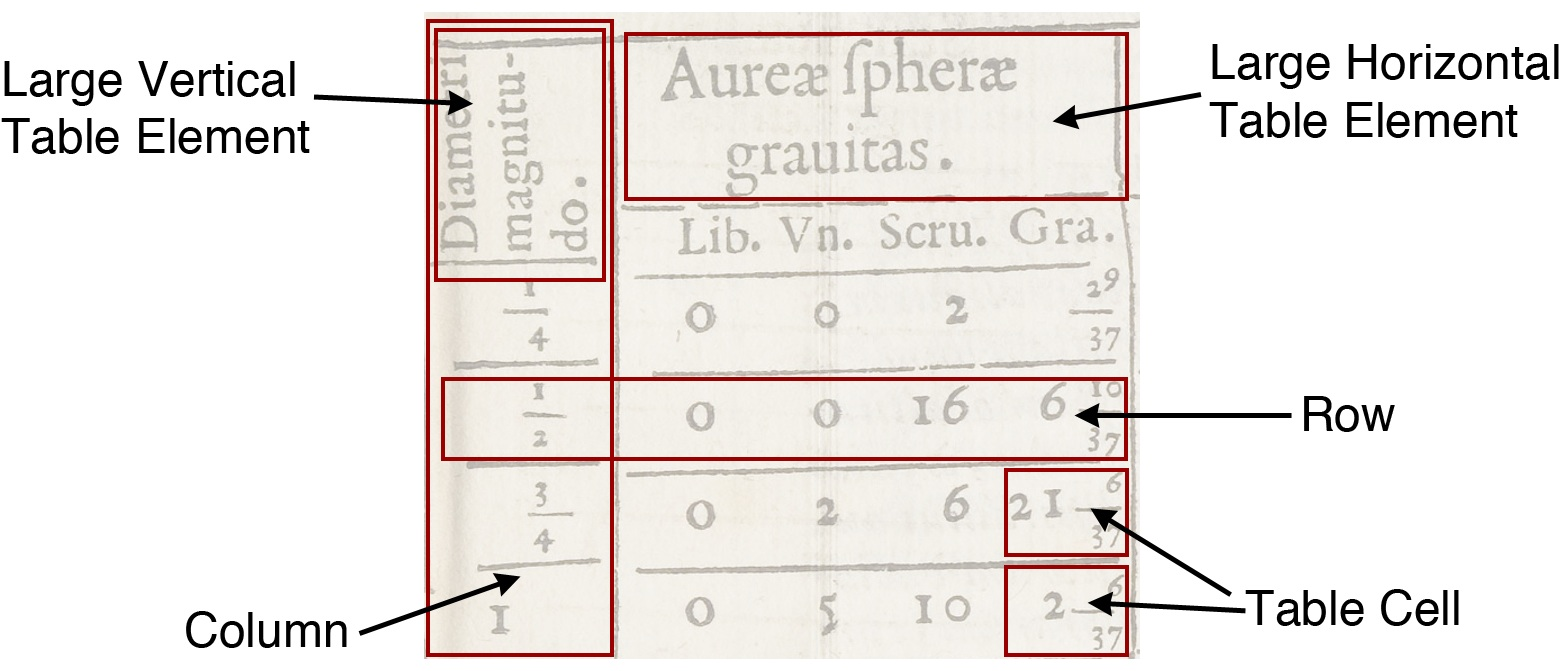
\includegraphics[width=\linewidth]{bettertable9}

\begin{crossref}
A transcription of this table can be found in \sect{section large vertical table elements}.
\end{crossref}

\vspace{3mm}
\begin{note}
In the context of tables, the term “column” refers to a vertical division in the table. The usage is different from the usage in \sect{section columns}. To avoid confusion, we will use the terms “table column” and “text column” in this section.
\end{note}

\subsubsection{Basic Rule}
\label{section tables basic rule}

\begin{mainrule}
A table is marked by §<tb>§ and §</tb>§. Use §#§ as cell separators. Type a return after each row. Do not type horizontal or vertical lines or large horizontal or vertical braces.
\end{mainrule}

\begin{clarification}
Type the §<tb>§ and §</tb>§ tags on separate lines. Do not treat the table columns as text columns (\sect{section columns}), i.e. do not type a whole column before you go on to the next column. If the whole table is in italics (\sect{section italics}), indicate this in the §<tb>§ tag, i.e. §<tb it>§.
\end{clarification}

\begin{sampleImage}{table_benedetti_439_2}

\begin{typeLatin}
\bold{<tb it>} \\
\bold{<col 1>} \\
Pag. \bold{#} Lin. \bold{#} Errata \bold{#} Correcta \\
3 \bold{#} 29 \bold{#} æqualis \bold{#} æquali \\
8 \bold{#} 35 \bold{#} maius \bold{#} maior \\
9 \bold{#} 15 \bold{#} in vnitate $uperficialis, erit ac \bold{#} in vnitate $upreficialis erit, ac \\
11 \bold{#} 1 \bold{#} proueuiens \bold{#} prouenientem \\
\someText \\
\bold{</col>} \\
\bold{<col 2>} \\
Pag. \bold{#} Lin. \bold{#} Errata \bold{#} Correcta \\
158 \bold{#} 26 \bold{#} ver$a \bold{#} ver$am \\
158 \bold{#} 26 \bold{#} $it \bold{#} $int \\
162 \bold{#} 22 \bold{#} cindenda \bold{#} $cindenda \\
163 \bold{#} 7 \bold{#} oppo$itus \bold{#} oppo$itum \\
\someText \\
\bold{</col>} \\
\bold{</tb>} 
\end{typeLatin}

If you are unsure whether the table in the example is divided into two text columns or not, use cell separators instead of §<col>§ tags:

\begin{typeLatin}
\bold{<tb it>} \\
Pag. \bold{#} Lin. \bold{#} Errata \bold{#} Correcta \bold{#} Pag. \bold{#} Lin. \bold{#} Errata \bold{#} Correcta \\
3 \bold{#} 29 \bold{#} æqualis \bold{#} æquali \bold{#} 158 \bold{#} 26 \bold{#} ver$a \bold{#} ver$am \\
8 \bold{#} 35 \bold{#} maius \bold{#} maior \bold{#} 158 \bold{#} 26 \bold{#} $it \bold{#} $int \\
\untranscribedText \\
\bold{</tb>}
\end{typeLatin}

\end{sampleImage}

\begin{crossref}
For §it§ see \sect{section italics}. The symbol §#§ is also used to mark large spaces in table-like structures (see \sect{section table-like structures}).
\end{crossref}


\subsubsection{Large Horizontal Table Elements}
\label{section large horizontal table elements}

\begin{mainrule}
Rule 1: In the case of a table element that horizontally spans more than one table cell, repeat the symbol §#§ before the table element for each cell spanned by the element, e.g. §####§ for an element spanning four cells. 
\end{mainrule}

\begin{clarification}
Do not type spaces between the §#§ symbols in this case. This rule applies even if the spanning element is the first element in a table row.
\end{clarification}

\begin{note}
In all other cases there should be a space before and after each §#§ symbol.
\end{note}

\vspace{3mm}
\begin{mainrule}
Rule 2: Within table cells, if text is broken into separate lines, do not type a return after the lines. Instead, type §\\§ to separate the lines.
\end{mainrule}

\vspace{3mm}
\begin{mainruleLessImportant}
Rule 3: If a table element spans the whole table width, type it as header/footer with §<h> </h>§ (without §#§, and do not use §\\§, but new lines).
\end{mainruleLessImportant}

\begin{sampleImage}{ghetaldi_p79_tabelle}

\begin{typeLatin}
\bold{<tb>} \\
\bold{<h>}Tabula ad inueniendam qualitatem \\
Auri, ex grauitate quam ha- \\
bet in aere & aqua.\bold{</h>}  \\
Qualitas \bold{\bs\bs} Auri. \bold{#} Grauitas Auri \bold{\bs\bs} in aere. \bold{####} Grauitas ... aqua. \bold{#} Mi$t\~u ... ære. \\
Part. \bold{#} Lib. \bold{#} Vnc. \bold{#} Scrup. \bold{#} Gran. \bold{#} Num. Fract. \bold{#} Part. \\
24 \bold{#} 1 \bold{#} 11. \bold{#} 8. \bold{#} 20. \bold{#} 372 \bold{#} 0 \\
23 \bold{#} 1 \bold{#} 11. \bold{#} 8. \bold{#} 5. \bold{#} 765 \bold{#} 1 \\
\someText \\
\bold{</tb>} \\
\bold{<tb>} \\
\bold{<h>}Tabella Partis pro \\
portionalis Deno- \\
minatorum Auri.\bold{</h>} \\
Pars proportio \bold{\bs\bs} nalis Auri in \bold{\bs\bs} partibus. 24. \bold{##} Differ\~etia ... aqua. \\
Part. \bold{#} Gran. \bold{#} Num: Fract. \\
1 \bold{#} 0. \bold{#} 1088 \\
2 \bold{#} 1. \bold{#} 409 \\
\someText \\
\bold{</tb>} \\
\end{typeLatin}

\end{sampleImage}


\subsubsection{Large Vertical Table Elements}
\label{section large vertical table elements}

\begin{mainrule}
Rule 4: If a table element vertically spans more than one cell, type its content in its uppermost cell. Mark each additional cell that belongs to this table element by~§"§.
\end{mainrule}

\vspace{3mm}
\begin{sampleImageSmall}{width=6cm}{ghetaldi_table}

\begin{typeLatin}
\bold{<tb>} \\
Diametri \bold{\bs\bs} magnitu- \bold{\bs\bs} do. \bold{####} Aureæ $pheræ \bold{\bs\bs} grauitas. \\
\bold{" #} Lib. \bold{#} Vn. \bold{#} Scru. \bold{#} Gra. \\
\bold{\{} 1/4 \bold{\}}  \bold{#} 0 \bold{#} 0 \bold{#} 2 \bold{#} \bold{\{} 29/37 \bold{\}} \\
\bold{\{} 1/2 \bold{\}}  \bold{#} 0 \bold{#} 0 \bold{#} 16 \bold{#} 6 \bold{\{} 10/37 \bold{\}} \\
\bold{\{} 3/4 \bold{\}}  \bold{#} 0 \bold{#} 2 \bold{#} 6 \bold{#} 21 \bold{\{} 6/37 \bold{\}} \\
1 \bold{#} 0 \bold{#} 5 \bold{#} 10  \bold{#} 2 \bold{\{} 6/37 \bold{\}}  \\
\bold{</tb>} \\
\end{typeLatin}
\end{sampleImageSmall}

\vspace{-5mm}
\begin{crossref}
For fractions such as §{1/4}§ see \sect{section fractions}.
\end{crossref}

\vspace{3mm}
\begin{note}
If the table elements vertically span the whole table and contain running text, they may not be table elements, but text columns (\sect{section columns}). If in doubt, check the example there.
\end{note}

% Rule about large curly braces? MH: nein


\tocspace
\subsection{Table-Like Structures}
\label{section table-like structures}

\subsubsection{Indexes}
\label{section indexes}

\begin{mainrule}
An index is marked by §<ind>§ and §</ind>§. Use §#§ for large spaces. Type a return after each row. 
\end{mainrule}

% Ob sie für jede Seite einen getrennten Index machen, sollen sie selbst entscheiden.


\begin{sampleImageSmall}[ 1]{width=10cm}{bacon_253}

\begin{typeLatin}
\bold{<ind it>} \\
Caterpillars \bold{#} \bold{_}153\bold{_} \\
Cements that grow hard \bold{#} \bold{_}183\bold{_} \\
Chalk, a good compo$t, \bold{_}122, 123\bold{_}. Good for \\
\bold{#} Pa$ture, as well as for Arable \bold{#} \bold{_}ibid\bold{_}. \\
Chameleons, \bold{_}80\bold{_}. Their nouri$hment, \bold{#} \bold{_}ibid\bold{_}. \\
\bold{#} A fond Tradition of them \bold{#} \bold{_}ibid\bold{_}. \\
\bold{</ind>} 
\end{typeLatin}
\end{sampleImageSmall}

\begin{crossref}
Within a structure in italics, the §_ _§ denote single words in upright type (see also \sect{section italics}).
\end{crossref}

\begin{sampleImage}[ 2]{gallac_91}

\begin{typeLatin}
\bold{<ind>} \\
\bold{<col 1>} \\
\someText \\
Diligenza $overchia, quale. \bold{#} 49 \\
Diminuzione di gro$$ezze, come deb- \\
\bold{#} ba condur$i. \bold{#} 56 \\
\bold{_}Diocleziano\bold{_}. Sue Terme. \bold{#} 51 \\
\someText \\
\bold{</col>} \\
\bold{<col 2>} \\
\someText \\
Errori di que$to genere, cagione di \\
\bold{#} tutti gli errori. \bold{#} 18. 19 \\
\bold{#} Provvedimenti dei Romani con- \\
\bold{#} tro a que$ti errori. \bold{#} 19 \\
\someText \\
\bold{</col>} \\
\bold{</ind>} \\
\end{typeLatin}
\end{sampleImage}


\subsubsection{Tables of Contents}
\label{section tables of contents}

\begin{mainrule}
A table of contents is marked by §<toc>§ and §</toc>§. Use §#§ for large spaces. Type a return after each row. 
\end{mainrule}

\begin{sampleImageSmall}[ 1]{width=12cm}{zubler_43_2}

\begin{typeLatin}
\bold{<toc it>} \\
Cap. 1. \bold{#} De Chorographia generatim: quid $it, & que ad eam In-\\
\bold{#} $trumenta poti{$s}imùm requi$ita, \bold{#} pag. 1. \\
II. \bold{#} De In$trumenti fabricâ, \bold{#} 2 \\
III. \bold{#} De Triangul{is}, omnium dimen$ionum fundamento, \bold{#} 5 \\
\someText \\
\bold{</toc>} 
\end{typeLatin}
\end{sampleImageSmall}


\begin{sampleImage}[ 2]{belidor_683}

\begin{typeLatin}
\bold{<toc it>} \\
\bold{_}CH\bold{<sc>}APITRE\bold{</sc>} I.\bold{_} Où l'on en$eigne comme $e fait la pou$$ée des \\
\bold{#} Voutes, & où l'on raporte quelques principes tirés de la méca- \\
\bold{#} nique pour en faciliter l'intelligence \bold{#} 2 \\
\bold{_}C\bold{<sc>}HAP\bold{</sc>}. II. \bold{_}De la maniere de calculer l'épai$$eur des Pié-droits \\
\bold{#} des Voutes en plain ceintre pour e$tre en équilibre par leur ré- \\
\bold{#} $i$tance avec la pou$$ée qu'ils ont à $oûtenir. \bold{#} 10 \\
\bold{</toc>} \\
\end{typeLatin}
\end{sampleImage}


\subsubsection{Large Spaces}

\begin{mainrule}
If a normal paragraph contains at least one large space, mark the paragraph by §#§ (i.e. §<p #>§) and mark each large space in the paragraph by §#§.
\end{mainrule}

\begin{clarification}
Before you use §<p #>§, make sure the paragraph is not part of a table, an index or a table of contents. In some texts the spaces after periods (“.”) is slightly larger than normal spaces; do not mark this.
\end{clarification}

\begin{sampleImageSmall}[ 2]{width=12cm}{Pappus_large_spaces}

\begin{typeLatin}
\bold{<p #>} \someText \\
extrema ad axes \bold{#} angulorum@ continent autem hunc propo$itiones \\
ferè exi$tentes vna multa, & varia theoremata, & linearum, & $uperficie- \\
rum, & $olidorum omnia $imul vna demon$tratione, & quæ nondum de- \\
mon$trata $unt, & quæ \bold{#} & in duodecimo libro horum elemento- \\
\someText \bold{</p>} \\
\end{typeLatin}
\end{sampleImageSmall}

%\subsubsection{Other Structures With Leading}
%Introduce a generic tag for leading: §<lead> # </lead>§ or so.
%Alternative: Section “Leading”, where leading is explained, with example. Then: toc's and indexes.
%One (weird) example would be Biancani 1635, p.195.
%Another semi-weird example: modern-style quotations. Alternatively in the block quotation section, or no rule at all.


\tocspace
\subsection{Notes}

\begin{note}
Handwritten notes (\sect{section handwritten notes}) are not transcribed. 
\end{note}

\subsubsection{Marginal Notes}
\label{section marginal notes}

\begin{mainrule}
A note in the left margin is marked by §<mgl> </mgl>§, and a note in the right margin is marked by §<mgr> </mgr>§. Type the marginal note on separate lines, starting after the line it is closest to. 
\end{mainrule}

\begin{clarification}
Do not mark paragraphs within a marginal note, i.e. do not use §<p> </p>§.
\end{clarification}

\begin{crossref}
For anchored marginal notes see \sect{section anchored marginal notes}.
\end{crossref}

\vspace{2mm}
\begin{sampleImage}[ 1: \, marginal notes in the left and right margins]{montag_mark_marginalnote_coimbricenses_232}

\notTranscribed

\vspace{2mm}
\end{sampleImage}

\begin{sampleImage}[ 2: \, transcribing a marginal note]{mkbsp_marginalnote_big_benedetti.jpg}

\begin{typeLatin}
\bold{<p>}
Si ad aliquã rectã lineã * compare\li{tur} parallelogrãm\bs\tld{}u, defici\bs\tld{}es forma\\
\bold{<mgr>}παραβληθῆ, \bold{_}ap\bold{_} \\
\bold{_}ponatur, appli-\bold{_} \\
\bold{_}cetur\bold{_</mgr>}\\
quadrata, ip$um cõparat\bs\tld{}u æqu\bs\tld{}u e$t ei quod (cõtine\li{tur}) $ub $egm\bs\tld{}etis\\
rect\li{ae} line\li{ae}, qu\li{ae} ex ip$a cõparatione $unt facta.
\bold{</p>}
\end{typeLatin}
\end{sampleImage}


\subsubsection{Footnotes}
\label{section footnotes}

\begin{mainrule}
Footnotes are marked by §<fn>§ and §</fn>§. Type the footnote where it appears on the page. Insert the footnote symbol or number in the §<fn>§ tag. The corresponding footnote symbol in the main text is marked by §<n>§. Insert the footnote symbol or number in the §<n>§ tag.
\end{mainrule}

\begin{clarification}
Ignore the superscript of the footnote symbol. Use §<n>§ in the main text only if you can identify the symbol as a footnote symbol and if there is a corresponding §<fn> </fn>§ tag somewhere. Do not mark paragraphs within a footnote, i.e. do not use §<p> </p>§. Do not type horizontal lines.
\end{clarification}

\begin{tabelle}[: \, common footnote symbols]
\begin{tabular}{llcccccc} \\
symbol && * & † & ‡ & \§ & ‖ & ¶ \\[2mm]
Unicode &&  \xs{U+002A} & \xs{U+2020} & \xs{U+2021} &\xs{U+00A7} & \xs{U+2016} & \xs{U+00B6} \\
\end{tabular}
\end{tabelle}

\vspace{2mm}
\begin{sampleImage}{montag_footnote2_euclid_264}
\begin{typeLatin}
\bold{<col 1>} \\
\bold{<h><n} *\bold{>} LEMMA.\bold{</h>}\\
\bold{<p>}Si fuerint tres rectæ lineæ in ratione aliqua,\\
erit ut prima ad tertiam ita rectangulum conten-\bold{</col>}\\
\bold{<col 2>} \\
\bold{<h>}* ΛΗΜΜΑ.\bold{</h>} \\
\bold{<p>}Εὰν ὦ\li{στι} τρ\li{εῖ}ς εὐθ\li{εῖ}\li{αι} \li{ἐν} λόγῳ \li{τι}νὶ, ἔ\li{σται} ὡς \\
ἡ \li{πρ}ώ\li{τη} \li{πρ}ὸς τ\li{ὴν} τ\li{ρί}\li{την} \li{οὕ}τως \li{τὸ} \li{ὑπὸ} τῆς\bold{</col>}\\
\bold{<fn} *\bold{>}Lemma hoc non agno$cunt \bold{_}Codd. MSS.\bold{_</fn>}
\end{typeLatin}
\end{sampleImage}

\begin{crossref}
For Greek ligatures see \sect{section greek ligatures}.
\end{crossref}

\begin{note}
If the footnote continues on the next page, close the first part with §</fn>§ before you go on to the next page. Mark the second part on the next page with new §<fn> </fn>§ tags.
\end{note}


\subsubsection{Anchored Marginal Notes}
\label{section anchored marginal notes}

\begin{mainruleLessImportant}
An anchored marginal note is marked by §<mgl> </mgl>§ or §<mgr> </mgr>§ according to its position and typed on separate lines starting after the line it is closest to (just like a normal marginal note). In addition, the anchor is treated like a footnote symbol, i.e. it is marked by §<n>§ in the main text and it is typed inside the §<mgl>§ or §<mgr>§ tag.
\end{mainruleLessImportant}

\begin{sampleImage}{montag_mark_anchor_marg_} % Euclid of Clavius 1607, p.795
\begin{typeLatin}
\bold{<p it>} \someText \\
circumferentiam datæ rectæ A, æqualem e$$e. Cùm enim $it, vt E,\\
ad A, ita B D, ad F G; hoc est, \bold{<n} \bold{_}a\bold{_}\bold{>} ita tota diameter circuli B C, ad\\
\bold{<mgr} a\bold{>}15.\\
\bold{_}quinti\bold{_}.\bold{</mgr>}\\
totam diametrum circuli F H: Sit autem vt diameter ad diametrum,\\
ita circumferentia B C, ad circumferentiam F H, vt Pappus demon- \\
\someText \bold{</p>}
\end{typeLatin}
\end{sampleImage}



\refstepcounter{subsubsection}
\label{section anchored comments}




\tocspace
\subsection{Printed Images}

\begin{note}
Treat handwritten figures in the same way as handwritten notes (\sect{section handwritten notes}), i.e. simply mark them by §<hd>§.
\end{note}


\subsubsection{Figures}
\label{section figures}

\begin{mainrule}
Where a figure occurs in the text, type §<fig>§ on a separate line. If you can identify a caption of the figure, mark it by §<cap> </cap>§. Additional text that describes parts of the figure is marked by §<desc> </desc>§. Use a single §<var> </var>§ tag for variable names and numbers. Type a closing §</fig>§ tag on a separate line after all §<cap>§, §<desc>§ and §<var>§ tags.
\end{mainrule}

\begin{clarification}
Type all §<cap>§, §<desc>§ and §<var>§ tags, in this order, on separate lines. 
%Type the caption on a separate line after <fig>. 
A figure may have more than one description. 
%Type each description on a separate line after <fig> and <cap>. 
If the same description is repeated in a figure, type it only once. 
%If the caption or a description is vertical, ignore this and type it as normal horizontal text. 
Separate the variable names and numbers in the §<var> </var>§ by spaces.
%If there are variable names or numbers in the figure, type them all in a single §<var> </var>§ tag.
Type §<fig/>§ instead of §<fig>§ and §</fig>§ to mark simple figures without §<cap>§, §<desc>§ or §<var>§ tags.
\end{clarification}

%(The rule that a caption may be typed above or below the §<fig>§ tag has disappeared.)

%(§</fig>§ makes sense only if there is at least one §<cap>§, §<desc>§ or §<var>§, so it would sometimes be used and sometimes not. Is this really a good idea? Check if there was any confusion with complex figures!)

\vspace{2mm}
\begin{sampleImageSmall}[ 1: \, a simple figure without caption, descriptions or variables]{width=7cm}{fig_sans_3}
\begin{typeLatin}
\bold{<p>} \someText \\
montre que vous placeriéz en cette façon \\
$ur une boule.\bold{</p>} \\
\bold{<fig/>} \\
\bold{<p>}Sous cette \bold{_}cornée\bold{_}, e$t \bold{_}l'iris\bold{_}, autre membrane, \\
\someText \bold{<p>} \\
\end{typeLatin}
\end{sampleImageSmall}

\vspace{2mm}
\begin{sampleImageSmall}[ 2: \, a figure with a caption]{width=12cm}{montag_imagewcaption}
\begin{typeLatin}
\bold{<p>} \someText \\
$e$quipedem, circumagito, ut altera pars æquè cale$cat ab igni.\bold{</p>}\\
\bold{<fig>} \\
\bold{<cap it>}Paruus Vncus ferreus.\bold{</cap>}\\
\bold{</fig>} \\
\bold{<p>}Præterea $i quando mi$tura $atis plumbi non habuerit, addito cum forci \\
\someText \bold{</p>}
\end{typeLatin}
\end{sampleImageSmall}

\begin{sampleImage}[ 3: \, figures with variables]{imageleftandright_4}
\begin{typeLatin}
\bold{<h it>_}E\bold{_}uclid. ex \bold{_}Z\bold{_}amb. \bold{_}T\bold{_}heorema \bold{_}68\bold{_}. \bold{_}P\bold{_}ropo$itio \bold{_}92\bold{_}.\bold{</h>} \\
\bold{<p>}Si areola comprehen$a fuerit $ub rationali & apotome $ecunda\\
\bold{<mgr>}92\bold{</mgr>}\\
quæ areolam pote$t, mediæ apotome e$t prima.\bold{</p>} \\
\bold{<fig>} \\
\bold{<var>}λ @ ο @ ν @ σ ξ χ @ τ μ\bold{</var>} \\
\bold{</fig>} \\
\bold{<p it>_}THEON\bold{_} ex \bold{_}Z\bold{_}ãb. \bold{_}A\bold{_}reola nãq; α β, \\
\bold{<fig>}\\
\bold{<var>}α @ @ ζ @ γ @ @ @ @\bold{</var>} \\
\bold{</fig>} \\
cõpreh\bs\tld{}edatur $ub ratiõali α γ, \& \bold{_}2\bold{_} a- \\
potome α δ. \bold{_}D\bold{_}ico \li{quod} quæ α β, areolam\\
pote$t, mediæ apotome e$t prima. \bold{_}E\bold{_}$to\\
enim (\li{per} 79 decimi) ip$i α δ cõgru\bs\tld{}es δ\\
\someText \bold{</p>}\\
\end{typeLatin}
\end{sampleImage}

\begin{sampleImageSmall}[ 4: \, figure with descriptions and variables]{width=8cm}{voltaire_156}
\begin{typeLatin}
\bold{<fig>} \\
\bold{<desc it>}Violet\bold{</desc>} \\
\bold{<desc it>}Pourpre\bold{</desc>} \\
\bold{<desc it>}Bleu\bold{</desc>} \\
\bold{<desc it>}Verd\bold{</desc>} \\
\bold{<desc it>}Jaune\bold{</desc>} \\
\bold{<desc it>}Orange\bold{</desc>} \\
\bold{<desc it>}Rouge\bold{</desc>} \\
\bold{<var>}A B C\bold{</var>} \\
\bold{</fig>} \\
\end{typeLatin}
\end{sampleImageSmall}


\subsubsection{Drop Caps}
\label{section drop caps}

\begin{mainrule}
Type a drop cap as an ordinary capital letter. 
\end{mainrule}

\begin{clarification}
Do not use a §<fig>§ tag (\sect{section figures}) for ornamental drop caps.
\end{clarification}

\vspace{2mm}
\begin{sampleImage}[ 1: \, a simple drop cap]{montag_mark_dropcap_unorna}
\begin{typeLatin}
\bold{<p>}FErunt Ari$tipp\bs~u tempe$tate maris ad incognita littora delatum, cum in are-\\
na vidi$$et qua$dã figuras geometricas delineatas exultant\bs\tld{}e l\li{ae}titia dixi$$e: Hæc\\ 
\someText \bold{</p>}
\end{typeLatin}
\end{sampleImage}

\begin{sampleImage}[ 2: \, an ornamental drop cap]{montag_mark_dropcap_orna}

\begin{typeLatin} 
\bold{<p>}LV\bold{<sc>}MEN\bold{</sc>} Lunæ etiam $i $it lumen reflexum Solis ab ip$a Luna, ab ea tamen\\
non ita reflectitur, vt à $uperficie polita $peculi, c\bs\tld{}u eius luminis tantã quã\\
titatem $uper ip$um corpus lunare videamus, & eo modo terminatã quo\\
con$picimus. per $e lumen, cau$a oculi e$t effectum, per accidens autem\\
puta quod vis. Terra deinde nunquam lunari lumine (quãuis $olaris reflexio exi$tat)\\ 
\someText \bold{</p>}
\end{typeLatin}
\end{sampleImage}

\vspace{-2mm}

\begin{crossref}
§<sc>§ marks small caps; see \sect{section small caps}. See also the example in \sect{Structural markup general example}.
\end{crossref}


\tocspace
\subsection{Handwritten Notes}
\label{section handwritten notes}

\begin{mainrule}
Handwritten notes are marked by §<hd>§. Do not type the note itself.
\end{mainrule}

\begin{clarification}
Type §<hd>§ on a separate line, after the line of the main text the note is closest to. 
\end{clarification}

\begin{sampleImage}[ 1: \, a handwritten note]{bsp_handwrittenmargin_2}

\begin{typeLatin}
\bold{<p>} \someText
h. $upponendo igitur in puncto. g. pondus, aut virtutem mouentem unius libræ, & in\\
h. duarum librarum, ab$\li{que} dubio hæ duæ uirtutes in huiu$modi di$tantijs à centro\\
\li{ae}quales inuic\bs\tld{}e er\bs\tld{}ut, ob rationes prioribus capitibus iam allatas, & $tatera orizontalis\\
\bold{<hd>}\\
manebit. Vnde clarum erit, \li{quod} quæuis etiam exigua virtus adiuncta ip$i. g. mouebit\\
$tateram extra orizontalem $itum. Nunc $i puncto. i. ex æquo medio inter. g. et. K.
\someText \bold{</p>}
\end{typeLatin}
\end{sampleImage}

\begin{sampleImage}[ 2: \, a handwritten note with a drawing]{mkbsp_handdrawing_euclid_515.jpg}
\begin{typeLatin}
\bold{<p>} \someText \\
ctè iuncta ad obtu$um angul\bs\tld{}u, à perp\bs\tld{}ediculari extrà depreh\bs\tld{}editur.\bold{</p>}\\
\bold{<hd>}
\end{typeLatin}

\end{sampleImage}

\begin{crossref}
Example 2 contains a signature and a catchword (\sect{section catchwords and signatures}), which are ignored.
\end{crossref}


\tocspace
\subsection{Unreadable Text}
\label{section unreadable text}

\subsubsection{Characters You are Unsure About}
\label{section characters you are unsure about}

\begin{mainrule}
If you are not sure about a character, type §<?>§ after it. If you are unsure about a whole paragraph, type §<?>§ directly after the §<p>§ tag, i.e. §<p><?>§. A completely unreadable character is typed as §@§. If it is unclear how many characters are unreadable, use §<gap>§ instead of §@§.
\end{mainrule}

\begin{clarification}
Use one §@§ for each unreadable character, e.g. §unr@@dable§. If in doubt, use §<gap>§, e.g. §unr<gap>dable§. If you are unsure about a group of characters, for example a whole word, do not type §<?>§ repeatedly for every character, e.g. type §word<?>§ rather than §w<?>o<?>r<?>d<?>§.
\end{clarification}

\vspace{2mm}
\begin{sampleImage}[ 1: \, a stain]{bsp_gaptag_circumcised} 
\begin{typeLatin}
\bold{<p>} \someText
d & f ad quadratum f, ergo di$iunctim erit quadratum \bold{@} ad\\
quadratum f, ergo b ad e $icut d ad f, item per æquam pro-\\ 
\someText \bold{</p>}
\end{typeLatin}

\end{sampleImage}

\begin{sampleImage}[ 2: \, a paper crease]{mkbsp_helptag.jpg}

\begin{typeLatin}
\bold{<p>} \someText
fe$$ore: cui acceptum feras quicquid hîc aut ad Gr\li{ae}cum exem\bold{<?>}plar, aut alio-\\
qui doctè re$titutum uideris. Adiecimus Phænomena, S\bold{@}ecularia, Pro-\\
theoriam Marini, & Data, argumentorum $imilitudine ind\bold{<?>}ucti. Quum\li{\bs´que}
\someText \bold{</p>}
\end{typeLatin}
\end{sampleImage}

\begin{crossref}
For unknown rather than unreadable characters please refer to \sect{section unknown characters}. 
\end{crossref}


\subsubsection{Unknown Characters}
\label{section unknown characters}

\begin{mainrule}
If there is an unknown character in the text, add it to the numbered
list of unknown characters. From then on, type its number whenever it
occurs in the text, e.g. §<001>§. Keep a separate list for every
single text. Do not make one list for the whole work order.
\end{mainrule}
 
\begin{clarification}
Before you create a number for an unknown character, first check whether \\
(1)~it is a known ligature (Latin: \sect{section latin ligatures}, Greek: \sect{section greek ligatures}), \\
(2)~it is a known symbol (appendix \ref{appendix list of all symbols}), \\
(3)~it is in the list of characters to be typed directly (\sect{section characters to be typed directly}), \\
(4)~there is a standard for typing it (\sect{section other diacritics}), or \\
(5)~it is already on the list of unknown characters.
 \end{clarification}

\begin{clarification}
If the character is indeed unknown: Assign the number §<001>§ to the first unknown character, §<002>§ to the second unknown character, and so on. Do not assign the same number twice. Use this number to type the unknown character. Always use the same number if the same unknown character occurs again. 
\end{clarification}

\begin{note}
Make sure that for a given text there is a single list containing all unknown characters, and that everyone uses this list. When the text is sent back to us, we will need a copy of this list. (See also \sect{section file conventions}.)
\end{note}

\begin{crossref}
For unreadable rather than unknown characters please refer to \sect{section characters you are unsure about}.
\end{crossref}

\subsubsection{Obvious Mistakes in the Text}
\label{section obvious mistakes}

\begin{mainrule}
If you have reason to believe that there is a mistake in the text, use §<!>§. 
\end{mainrule}

\begin{clarification}
Do not silently correct the mistake.
\end{clarification}

\vspace{3mm}
\begin{example}[: \, wrong numbering of anchored marginal notes]

\vspace{-5mm}
\begin{typeLatin}
\bold{<mgl} a\bold{>} ... \bold{</mgl>} \\
\bold{<mgl} b\bold{>} ... \bold{</mgl>} \\
\bold{<mgl} c\bold{>} ... \bold{</mgl>} \\
\bold{<mgl} e\bold{><!>} ... \bold{</mgl>} \\
\end{typeLatin}
\end{example}


\section{Latin Alphabet}

\tocspace
\subsection{General}
\label{section latin general}

\subsubsection{Punctuation}
\label{section latin punctuation}

\begin{mainrule}
Type a space after the punctuation marks § . , : ; ! ?§ \quad 
Type a space before the opening brackets § ( [ § and after the closing brackets  § ) ] §.
\end{mainrule}

\begin{clarification}
Ignore superfluous and missing spaces before and after punctuation marks and brackets.
\end{clarification}

\vspace{2mm}
\begin{sampleImage}[ 1: \, normal punctuation marks]{montag_punctuation}
\begin{typeLatin}
\bold{<p>}Exempli gratia, $umemus quadratum. \bold{_}3\bold{_}. $cilicet 9. quod in $ummam cum qua-\\
drato. 4. colligemus, nempè. 1\bold{_}6\bold{_}. erit\bs'q; quadratum. 25. & ita quadratum. 6. hoc e$t.\\
\bold{_}36\bold{_}. collectum cum quadrato. 8. nempè. \bold{_}6\bold{_}4. efficiet quadratum. 100. ita etiam qua-\\
dratum. \bold{_}9\bold{_}. hoc e$t. 81. coniunctum quadrato. 12. nempè. 144. producet quadra- \\
\someText \bold{</p>}
\end{typeLatin}
\end{sampleImage}

\begin{sampleImage}[ 2: \, unusual punctuation marks]{punktuation_2}
\begin{typeLatin}
\bold{<p>} \someText
$cindendus pannus uel tela: num id $ine cultro uel forfice faciet? num con-\\
$uet ullam ue$tem $ine acu? ne populus quidem tran$marinus pennarum\\
contextu corporis tegumentum faciet $ine \li{ij}$dem in$trumentis, nec pel-\\ 
\someText \bold{</p>}
\end{typeLatin}
\end{sampleImage}


\subsubsection{Hyphens}
\label{section hyphens}

\begin{mainrule}
If the line ends with a hyphen, type it.
\end{mainrule}

\begin{clarification}
Hyphens at the end of a line can have different shapes. Always type a normal hyphen § - § regardless of its actual shape in the text. %Do not insert a space at the end of the line. 
\end{clarification}

\vspace{2mm}
\begin{sampleImage}[ 1: \, normal hyphen]{hyphen_normal} 
\begin{typeLatin}
Oportet autem arcum in maiore circulo datum non e$-
\end{typeLatin}
\end{sampleImage}

\begin{sampleImage}[ 2: \, slanted hyphen]{montag_hyphen_single_slanted} 
\begin{typeLatin}
æqualia. 4 Et $i ab inæqualibus æqualia demas, quæ relinquun-
\end{typeLatin}
\end{sampleImage}

\begin{sampleImage}[ 3: \, slanted double hyphen]{hyphen_doppelt_schraeg} 
\begin{typeLatin}
RENSIS CLARISSIMI PHILOSOPHI, MATHEMA-
\end{typeLatin}
\end{sampleImage}

\subsubsection{Dashes}
\label{section dashes}

\begin{mainrule}
Type the en dash – and the em dash — directly as Unicode characters.
\end{mainrule}

\begin{clarification}
The en dash – (U+2013) is longer than the normal hyphen. The em dash — (U+2014) is longer than the hyphen and the en dash.
\end{clarification}

\tocspace
\subsection{Characters}

\subsubsection{Characters to be Typed Directly}
\label{section characters to be typed directly}

\begin{mainrule}
If a character with diacritics can be easily typed and encoded as a single Unicode character, type it directly.
\end{mainrule}

\mehrzeilen[-2]

\vspace{2mm}
\begin{liste}[: \, characters that can be typed directly]

\vspace{-4mm}
\begin{longtable}[l]{c@{ }lc@{ }lc@{ }lc@{ }lc@{ }lc@{ }l}
\multicolumn{12}{l}{\s Characters with acute accent} \\[2mm]
á & \xs{(U+00E1)} & é & \xs{(U+00E9)} & í & \xs{(U+00ED)} & ó & \xs{(U+00F3)} & ú & \xs{(U+00FA)} && \\
Á & \xs{(U+00C1)} & É & \xs{(U+00C9)} & Í & \xs{(U+00CD)} & Ó & \xs{(U+00D3)} & Ú & \xs{(U+00DA)} && \\ 
\\
\multicolumn{12}{l}{\s Characters with grave accent} \\[2mm]
à & \xs{(U+00E0)} & è & \xs{(U+00E8)} & ì & \xs{(U+00EC)} & ò & \xs{(U+00F2)} & ù & \xs{(U+00F9)} && \\
À & \xs{(U+00C0)} & È & \xs{(U+00C8)} & Ì & \xs{(U+00CC)} & Ò & \xs{(U+00D2)} & Ù & \xs{(U+00D9)} && \\ 
\\
\multicolumn{12}{l}{\s Characters with circumflex accent} \\[2mm]
â & \xs{(U+00E2)} & ê & \xs{(U+00EA)} & î & \xs{(U+00EE)} & ô & \xs{(U+00F4)} & û & \xs{(U+00FB)} && \\
 & \xs{(U+00C2)} & Ê & \xs{(U+00DA)} & Î & \xs{(U+00CE)} & Ô & \xs{(U+00D4)} & Û & \xs{(U+00DB)} && \\ 
\\
\multicolumn{12}{l}{\s Characters with umlaut/diaeresis} \\[2mm]
ä & \xs{(U+00E4)} & ë & \xs{(U+00EB)} & ï & \xs{(U+00EF)} & ö & \xs{(U+00F6)} & ü & \xs{(U+00FC)} & ÿ & \xs{(U+00FF)} \\
Ä & \xs{(U+00C4)} & Ë & \xs{(U+00CB)} & Ï & \xs{(U+00CF)} & Ö & \xs{(U+00D6)} & Ü & \xs{(U+00DC)} & Ÿ & \xs{(U+0178)} \\ 
\\
\multicolumn{12}{l}{\s Characters with tilde} \\[2mm]
ã & \xs{(U+00E3)} & õ & \xs{(U+00F5)} & ñ & \xs{(U+00F1)} &&& \\
à & \xs{(U+00C3)} & Õ & \xs{(U+00D5)} & Ñ & \xs{(U+00D1)} &&& \\ 
\\
\multicolumn{12}{l}{\s Characters with cedilla} \\[2mm]
ç & \xs{(U+00C7)} &&&&& \\
Ç & \xs{(U+00E7)} \\ 
\\
\multicolumn{12}{l}{\s Common ligatures} \\[2mm]
æ & \xs{(U+00C6)} & œ & \xs{(U+0153)} \\
Æ & \xs{(U+00E6)} & Œ & \xs{(U+0152)} \\
\end{longtable}
\end{liste}

\begin{note}
Type the character ſ (i.e. long s) as §$§.
\end{note}

\begin{note}
The small letter i sometimes occurs without the dot above. Type it as a normal §i§. 
\end{note}

\vspace{2mm}
\begin{sampleImageSmall}[: \, long s, dotless i]{height=8mm}{dotlessi_euclidclavius_13}
\begin{typeLatin}
o$tendit \\
\end{typeLatin}
\end{sampleImageSmall}

\vspace{-3mm}
\begin{crossref}
For the ligature §$t§ see \sect{section latin ligatures}.
\end{crossref}

\subsubsection{Other Diacritics}
\label{section other diacritics}

\begin{mainrule}
If a character cannot be typed directly but is a combination of a known character and a known diacritic, type \bs\,, then the diacritic, then the character.
\end{mainrule}

\begin{clarification}
Use this method only if the character is not in the list in \sect{section characters to be typed directly}.
\end{clarification}

\begin{tabelle}[: \, how to type diacritics]

\begin{tabular}{@{}ccc@{ }ccc@{}ccccc@{}}
&& circum- & umlaut/ && &&& dot\\
acute & grave & flex & diaeresis & tilde & cedilla &&& above & macron & breve \\[1mm]
\hline &&&& &&&& \\
\'q & \`q &  \^q & \"q & \~q & {\fontspec{Helvetica}{\c{e}}} &&& {\fontspec{Helvetica}{\.a}} & q̄ & ĕ \\[2mm]
§\'q§ & §\`q§ & §\^q§ & §\"q§ & §\~q§ & §\,e§ &&& §\.a§ & §\=q§ & §\-e§ \\ \\
\end{tabular}
\end{tabelle}

\begin{example}


\includegraphics[height=8mm]{aeqtildeles}

\vspace{-3mm}
\begin{typeLatin}
æ\bs~qles
\end{typeLatin}

\end{example}

\begin{note}
\k{e} (e with ogonek) and \r{q} (q with ring) are treated as ligatures; see \sect{section latin ligatures}.
\end{note}


\tocspace
\subsection{Type Styles}

\subsubsection{Italics}
\label{section italics}

\begin{mainrule}
Use underscores §_ _§ to mark the beginning and end of words or whole lines in italics. Encode only up to a few lines of text this way, enclosing each line in underscores. A whole paragraph in italics is marked by §it§ in the §<p>§ tag, i.e. §<p it>§. Also, be careful not to include punctuation marks.
\end{mainrule}

\begin{clarification}
This applies not only to paragraphs (\sect{section paragraphs}), but also to tables (\sect{section tables}), i.e. §<tb it>§, and pages (\sect{section page breaks}), i.e. §<pb it>§. If you use §it§, do not mark the lines with additional §_ _§ to indicate italics. However, within a §<p it>§ paragraph you can use §_ _§ to mark single words in upright type (see §_THEON_§ in example 2 in \sect{section figures}).
\end{clarification}

\begin{sampleImageSmall}[ 1: \, a single word in italics]{scale=0.25}{montag_kursiv2}
\begin{typeLatin}
C\bold{<sc>}AMPANI\bold{</sc>} \bold{_}annotatio\bold{_}. Habito minimo, $i cura e$t
\end{typeLatin}
\end{sampleImageSmall}

\begin{sampleImage}[ 2: \, a phrase in italics, including a line break]{italics_intwolines}
\begin{typeLatin}
\bold{<p>} \someText\\
bus, figuris vtar geometricis, ita enim in .2. libr. fecit Euclides, qui mo-\\
dus, eo magis mihi arridet, quo minus e$t ab$tractus, \bold{_}quoniam oportet in-\bold{_}\\
\bold{_}telligentem phanta$mata $peculari\bold{_}, cum pr\li{ae}terea per$picuum $it, di$cretum\\
omne, ex continui diui$ione aliquo modo oriri, $iue actu, $iue potentia.\\
\someText \bold{</p>}
\end{typeLatin}
\end{sampleImage}


\subsubsection{Bold Face}
\label{section bold face}

\begin{mainruleLessImportant}
Use §<bf> </bf>§ to mark bold face.
\end{mainruleLessImportant}

\begin{example} 

\vspace{-4mm}
This is a \textbf{bold}  statement.

\begin{typeLatin}
This is a \bold{<bf>}bold\bold{</bf>} statement.
\end{typeLatin}
\end{example}

\subsubsection{Small Caps}
\label{section small caps}

\begin{mainrule}
If you can identify capital letters as small caps, use §<sc> </sc>§. 
\end{mainrule}

\vspace{3mm}
\begin{sampleImageSmall}{scale=0.2}{small_caps_euclid_515}

\begin{typeLatin}
\bold{<p>}C\bold{<sc>}AMPANVS\bold{</sc>}. Sit datus trigonus\\
a: cui nos uolumus æquum quadra-\\
tum de$cribere. De$ignabo $uperfici\bs\tld{}e \\
\someText \bold{</p>} \\
\end{typeLatin}

\end{sampleImageSmall}

%\mehrzeilen

\subsubsection{Subscript and Superscript}
\label{section subscript and superscript}

\begin{mainrule}
Use §<_>§ and §</_>§ for subscript. Use §<^>§ and §</^>§ for superscript.
\end{mainrule}

\begin{example}[ 1: \, subscript]

\vspace{-4mm}
Assume that a$_1$ is negative.
\begin{typeLatin}
Assume that a\bold{<_>}1\bold{</_>} is negative.
\end{typeLatin}
\end{example}

\begin{example}[ 2: \, superscript]

\vspace{-4mm}
The square x$^2$ is always non-negative.
\begin{typeLatin}
The square x\bold{<^>}2\bold{</^>} is always non-negative.
\end{typeLatin}
\end{example}

\begin{note}
Please be sure to distinguish between subscript and superscript.
\end{note}

\begin{note}
Numbers or other symbols in superscript may indicate a footnote (\sect{section footnotes}). Check whether there is a corresponding footnote somewhere.
\end{note}

\subsubsection{Underlines and Overlines}
\label{section underlines and overlines}

\begin{mainrule}
Underlines, i.e. lines below characters or words, are marked by §<ul> </ul>§. 
Overlines, i.e. lines above characters or words, are marked by §<ol> </ol>§. 
\end{mainrule}

% Examples (from the Formax questions: Cavalieri 1653: Special instruction was to use §{ 00 / }§ (p.0157) and §{ / 1 }§ (p.0354); now we tell them to use §<ol>§ and §<ul>§. But would this really be a good idea in a situation as in Cavalieri? The idea of overlines and underlines is that the letters look normal and there is simply a line added above or below the letters. In Cavalieri, however, the lines make the characters move up or down. $\to$ still a Special Instruction, and not a good example here.)

\vspace{3mm}
\begin{example}[ 1: \, underlines]

\vspace{-4mm}
In this sentence, \underline{two words} are underlined.

\vspace{-3mm}
\begin{typeLatin}
In this sentence, \bold{<ul>}two words\bold{</ul>} are underlined. \\
\end{typeLatin}
\end{example}

\begin{sampleImageSmall}[ 2: \, overlines]{height=8mm}{overlines}

\begin{typeLatin}
\bold{<ol>}D E\bold{</ol><^>}3\bold{</^>} ad \bold{<ol>}A C\bold{</ol><^>}3\bold{</^>}, ita Cohærentia \\
\end{typeLatin}
\end{sampleImageSmall}

\begin{crossref}
In mathematical formulas, an overline may also indicate a root (see \sect{section roots}).
\end{crossref}


\subsubsection{Text in Red}
\label{section text in red}

\begin{mainruleLessImportant}
Text in red is marked by §<red>§ and §</red>§. 
\end{mainruleLessImportant}

\vspace{3mm}
\begin{sampleImageSmall}{width=12cm}{red_euclid_5enhanced}

\begin{typeLatin}
\bold{<h it><red>}OMNES PERSPICVIS DEMONSTRA-\bold{</red>} \\
tionibus, accurati$que $choli\li{is} illu$trati: nunc quartò editi, \\
ac multarum rerum acce\li{$s}ione post primam \\
editionem locupletati.\bold{</h>} \\
\end{typeLatin}
\end{sampleImageSmall}

\subsubsection{Vertical Text}

\begin{mainrule}
Type vertical text as you would type horizontal text. The vertical text is not explicitly marked as such.
\end{mainrule}

\begin{crossref}
For an example of vertical text see the example in \sect{section large horizontal table elements}.
\end{crossref}


\tocspace
\subsection{Latin Ligatures}
\label{section latin ligatures}

\begin{mainrule}
Resolve easy ligatures silently. Resolve difficult ligatures too, but type §{§ and §}§ around them.
\end{mainrule}

\begin{crossref}
Do not resolve æ and œ (see \sect{section characters to be typed directly}).
\end{crossref}

\vspace{2mm}
\begin{liste}[ 1: \, easy ligatures]

\begin{tabular}{@{}lccccccccccc}
upright & \lig{ff} & \lig{fi} & \lig{fl} & \lig{ffi} & \lig{ffl} & \lig{ſſ} & \lig{ſi} & \lig{ſſi} & \lig{ſt} & \lig{st} & {\fontspec[Ligatures=Rare]{Hoefler Text} \Large ct} \\[2mm] % siehe fontspec.pdf, Abschnitt "Ligatures"
italics & \lig{\textit{ff}} & \lig{\textit{fi}} & \lig{\textit{fl}} & \lig{\textit{ffi}} & \lig{\textit{ffl}} & \lig{\textit{ſſ}} & \lig{\textit{ſi}} & \lig{\textit{ſſi}} & \lig{\textit{ſt}} & \lig{\textit{st}} & {\fontspec[Ligatures=Rare]{Hoefler Text} \Large \textit{ct}} \\[2mm] % siehe fontspec.pdf, Abschnitt "Ligatures"
& §ff§ & §fi§ & §fl§ & §ffi§ & §ffl§ & §$$§ & §$i§ & §$$i§ & §$t§ & §st§ & §ct§ \\ \\ 
\end{tabular}
\end{liste}

\begin{liste}[ 2: \, difficult letter ligatures]
\begin{tabular}{lllllllllll} 
\\

\includegraphics[height=8mm]{ij_ligatur} & §{ij}§ &&

\includegraphics[height=8mm]{is_ligature} & §{is}§ &&
%\includegraphics[height=8mm]{ss_ligature} &
{\Large ß} & \textit{\Large ß} & §{$s}§ 
\\ \\
\end{tabular}
\end{liste}

%\newpage

\begin{liste}[ 3: \, difficult complex ligatures]
\begin{longtable}[l]{lllllllllll} 

\includegraphics[height=8mm]{eogonek} & §{ae}§ \\ \\

\includegraphics[height=8mm]{colnr} & §{con}§ 
\\ \\

\includegraphics[height=8mm]{q3} & §{que}§ 
&

\includegraphics[height=8mm]{q3tilde} & §{quam}§ 
&&
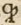
\includegraphics[height=8mm]{qmitslash} & §{quis}§ 
&&

\includegraphics[height=8mm]{qmitkreis} & §{quo}§ 
\\ \\

\includegraphics[height=8mm]{p_stroke} & §{per}§ 
\\ \\
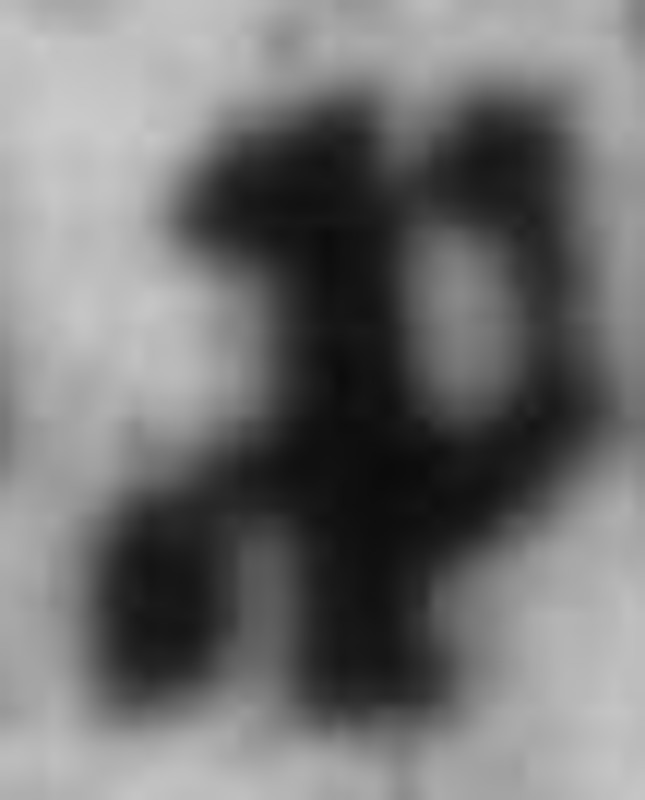
\includegraphics[height=8mm]{p} & §{pro}§ 
\\ \\
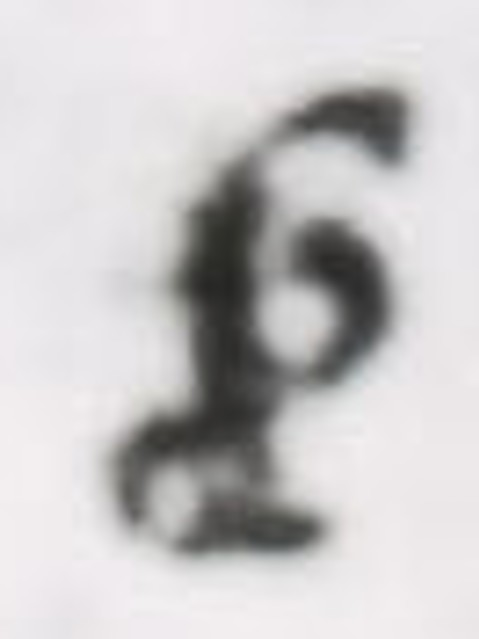
\includegraphics[height=8mm]{longs_p_slash} & §{secundu}§ 
\\ \\

\includegraphics[height=8mm]{t_with_curly_bar} & §{tur}§
\end{longtable}
\end{liste}

\begin{example}[ 1: \, words containing easy ligatures]


\includegraphics[height=8mm]{neulig_fi} \quad

\includegraphics[height=8mm]{neulig_st} \quad

\includegraphics[height=8mm]{neulig_ct}

\vspace{-3mm}
\begin{typeLatin}
$cientificè     \bold{_}stater\bold{_}     effectibus
\end{typeLatin}


\includegraphics[height=8mm]{bsp_ligst_benedetti_13} \quad

\includegraphics[height=8mm]{neulig_longsi} \quad

\includegraphics[height=8mm]{bsp_ligss_benedetti_13} \quad

\includegraphics[height=8mm]{neulig_longssi}

\vspace{-3mm}
\begin{typeLatin}
po$teris        occa$ione          e$$e     Sereni$$imo
\end{typeLatin}

\end{example}

\begin{example}[ 2: \, words containing difficult ligatures]


\includegraphics[height=8mm]{accessione}

\vspace{-3mm}
\begin{typeLatin}
\bold{_}acce\li{$s}ione\bold{_}
\end{typeLatin}


\includegraphics[height=8mm]{neulig_que} \quad

\includegraphics[height=8mm]{duoque} \quad

\includegraphics[height=8mm]{neulig_quod} \quad
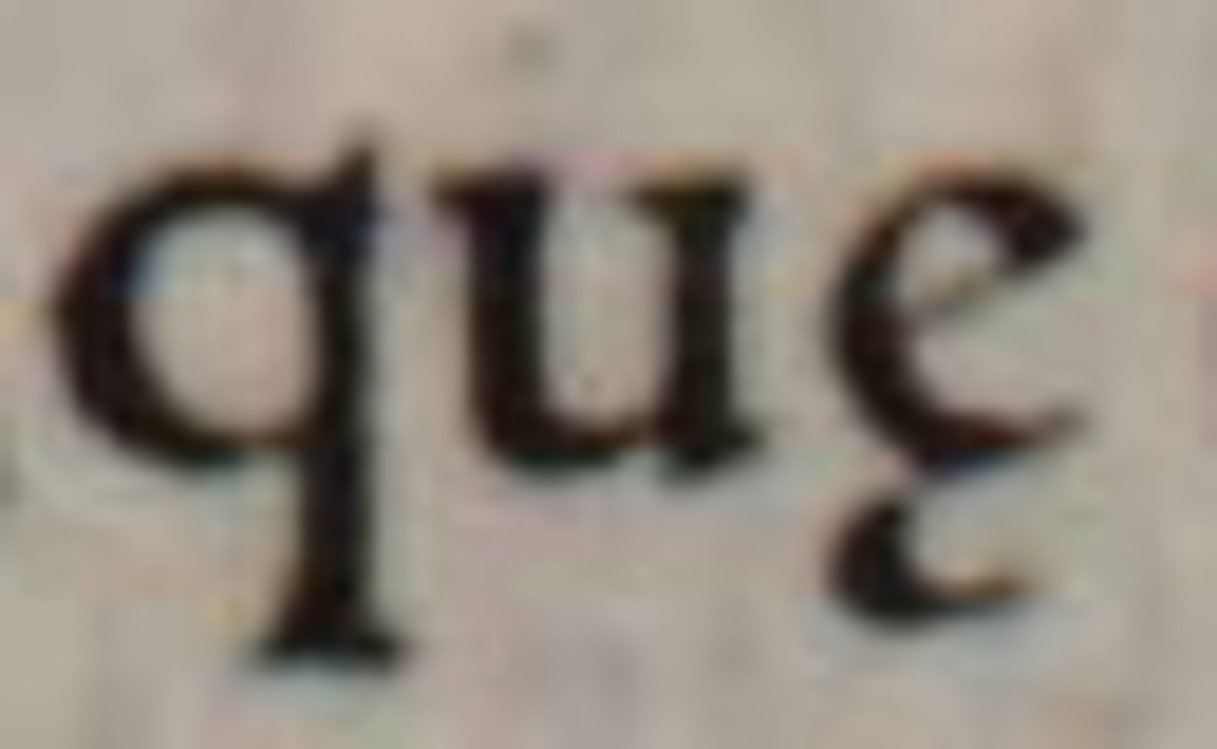
\includegraphics[height=8mm]{queogonek} \quad
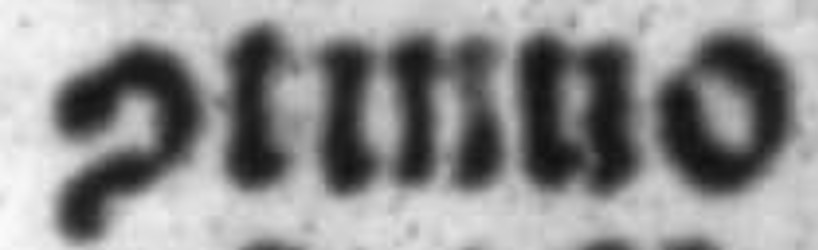
\includegraphics[height=8mm]{continuo} \quad

\includegraphics[height=8mm]{probo} \quad

\includegraphics[height=8mm]{longsm_secundum}

\vspace{-3mm}
\begin{typeLatin}
utriu$\li{que}    duo'\li{que}   \li{quo}d  qu\li{ae}    \li{con}tinuo      \li{pro}bo   \li{secundu}m
\end{typeLatin}

\end{example}


\tocspace
\subsection{Additional Rules for Specific Languages}

\subsubsection{German}

\begin{mainrule}
In German text, type the characters ä, ö, ü and ß directly as Unicode characters.
\end{mainrule}

\vspace{3mm}
\begin{tabelle}[: \, German characters]

\vspace{-1mm}
\begin{tabular}{@{}lccclc}
small letters \hspace{8mm} & ä & ö & ü && ß \\[2mm]
Unicode & \xs{U+00E4} & \xs{U+00F6} & \xs{U+00FC} && \xs{U+00DF} \\[4mm]
capital letters \hspace{8mm} & Ä & Ö & Ü \\[2mm]
Unicode & \xs{U+00C4} & \xs{U+00D6} & \xs{U+00DC} \\[3mm]
\end{tabular}
\end{tabelle}

\begin{note}
The umlauts ä, ö, and ü are already supposed to be typed directly; see the list in \sect{section characters to be typed directly}. Only the character ß is new here. In non-German text you can still type it as §{$s}§, see \sect{section latin ligatures}.
\end{note}

\begin{crossref}
For German text in Fraktur see \sect{section fraktur}.
\end{crossref}


\section{Greek Alphabet}

\tocspace
\subsection{Characters}

\begin{mainrule}
Type Greek characters directly as Unicode characters. 
\end{mainrule}

\begin{clarification}
Type characters with diacritics as precomposed characters from the Unicode Greek Extended block, i.e. §ἀ§ as the Unicode character U+1F00, etc.
\end{clarification}


\tocspace
\subsection{Punctuation}
\label{section greek punctuation}

\begin{mainrule}
The rules for Latin punctuation apply. In addition, type the mid-dot §·§ directly.
\end{mainrule}

\begin{clarification}
The mid-dot §·§ (Greek ano teleia) has the Unicode codepoint U+0387. 
\end{clarification}

\begin{crossref}
For the Latin punctuation see \sect{section latin punctuation}.
\end{crossref}


\tocspace
\subsection{Greek Ligatures}
\label{section greek ligatures}

\begin{mainrule}
Resolve letter variations silently. Resolve all ligatures and type §{§ and §}§ around them. If a ligature contains some diacritics, type them. 
\end{mainrule}

\begin{clarification}
The acute accent above §ι§, e.g. in §{τί}§, may be vertical; in this case type it as an acute accent. In some ligatures the accent is not above the correct character; type the accent above the vowel (§α§, §ε§, §η§, §ι§, §ο§, §υ§, §ω§), e.g. §{μέν}§. In two-letter ligatures of two vowels, type the accent above the second letter, e.g. §{οὕ}§. In some ligatures the accent is not clearly visible; if the resolved version in the list contains an accent, type it. In Greek texts, the circumflex has two shapes (circumflex~§^§ and tilde~§~§); always type it as normal circumflex. Type the end-sigma §ς§ directly, i.e. do not treat it as a letter variation.
\end{clarification}

\newcommand{\phlk}[1]{\textphlk{\LARGE #1}}
\newcommand{\phlktbl}[1]{\textphlk{\LARGE #1} & §\{#1\}§}

\vspace{3mm}
\begin{liste}[ 1: \, letter variations]

\vspace{-3mm}
\begin{tabular}{ccccc}
{\Large ϐ} && {\Large ϖ} && {\fontspec{Rgreekl2} \large õ} \\[2mm] % U+03D0, U+03D6 
§β§ && §π§ && §τ§ \\[2mm]
\end{tabular}
\end{liste}

\begin{liste}[ 2: \, two-letter ligatures]

\phlk{αι} 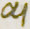
\includegraphics[height=6mm]{ai} §{αι}§ \quad
\phlk{ἀν}  §{ἀν}§ \quad
\phlk{αύ} §{αύ}§ \\

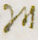
\includegraphics[height=6mm]{gE} §{γη}§ \quad

\includegraphics[height=6mm]{gr} §{γρ}§ \quad
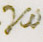
\includegraphics[height=6mm]{gO} §{γω}§ \\


\includegraphics[height=6mm]{di_A} §{δί}§ \quad
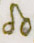
\includegraphics[height=6mm]{do} §{δο}§ \quad
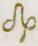
\includegraphics[height=6mm]{dr} §{δρ}§ \\

\phlk{ει} 
\includegraphics[height=6mm]{ei} §{ει}§ \quad
\phlk{εῖ} \, {\fontspec{Rgreekl2} \Large Ƭ} §{εῖ}§ \quad
\phlk{εν}  §{εν}§ \quad
\phlk{ευ} 
\includegraphics[height=6mm]{eu} §{ευ}§ \\

\phlk{ην} §{ην}§ \quad

\includegraphics[height=6mm]{En_G} §{ὴν}§ \\


\includegraphics[height=6mm]{tha} §{θα}§ \quad
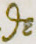
\includegraphics[height=6mm]{the} §{θε}§ \\


\includegraphics[height=6mm]{ko} §{κο}§ \\

\phlk{λλ} 
\includegraphics[height=6mm]{ll} §{λλ}§ \\


\includegraphics[height=6mm]{mo} §{μο}§ \\


\includegraphics[height=6mm]{pa} §{πα}§ \quad

\includegraphics[height=6mm]{po} §{πο}§ \quad
\includegraphics[height=6mm]{p-} §{πτ}§ \\

%\phlk{έξ} \phlk{ἒξ}  §{όξ}§ \quad
\phlk{όξ} \phlk{ὄξ}  §{όξ}§ \quad
\phlk{ου} \includegraphics[height=6mm]{ou} §{ου}§ \\
 
\phlk{ρί} \includegraphics[height=6mm]{ri} §{ρι}§ \\

\phlk{σθ}  §{σθ}§ \quad
\includegraphics[height=6mm]{si} §{σι}§ \quad
\includegraphics[height=6mm]{sk} §{σκ}§ \quad
\phlk{σσ}  §{σσ}§ \quad
\phlk{στ} \includegraphics[height=6mm]{st} §{στ}§ \quad
\phlk{σχ} §{σχ}§ \\

\includegraphics[height=6mm]{ta} §{τα}§ \quad
\includegraphics[height=6mm]{te} §{τε}§ \quad
\includegraphics[height=6mm]{ti} §{τι}§ \quad
\includegraphics[height=6mm]{ti_A} §{τί}§ \quad
\includegraphics[height=6mm]{to} §{το}§ \quad
\includegraphics[height=6mm]{tr} §{τρ}§ \\

\phlk{υν} \includegraphics[height=6mm]{un} §{υν}§ \\

\phlk{χρ} \includegraphics[height=6mm]{chr} §{χρ}§ \\

\includegraphics[height=6mm]{psi} §{ψι}§ \\

\end{liste}


\begin{note}
Some two-letter ligatures have different shapes within a word and as a separate word, e.g. §{εν}§ as a two-letter ligature (table 2) and §{ἐν}§ as a word ligature (table 4).
\end{note}


\begin{liste}[ 3: \, ligatures of three or more letters]

\includegraphics[height=6mm]{men} §{μεν}§ \quad
\includegraphics[height=6mm]{men_A} §{μέν}§ \\

\includegraphics[height=6mm]{pro} §{προ}§ \\

\phlk{στί} \includegraphics[height=6mm]{sti} §{στι}§ \quad
\includegraphics[height=6mm]{sto} §{στο}§ \\

\end{liste}


\begin{liste}[ 4: \, word ligatures]

\includegraphics[height=6mm]{apo_SL_G} §{ἀπὸ}§ \\

\phlk{γάρ} §{γὰρ}§ \\

\phlk{δια} \includegraphics[height=6mm]{dia_G} §{διὰ}§ \\

\includegraphics[height=6mm]{en_SL} §{ἐν}§ \quad
\includegraphics[height=6mm]{epi_SL_G} §{ἐπὶ}§ \\

\phlk{καὶ} \includegraphics[height=6mm]{kai_G} \,
\phlk{κι} \includegraphics[height=6mm]{and} §{καὶ}§ \quad
\phlk{κατὰ} §{κατὰ}§ \\

\phlk{μετὰ} \includegraphics[height=6mm]{meta_G} §{μετὰ}§ \\

\includegraphics[height=6mm]{tEn_G} §{τὴν}§ \quad
\phlk{τῶν} \includegraphics[height=6mm]{tOn_C} §{τῶν}§ \\

\includegraphics[height=6mm]{upo_SA_G} §{ὑπὸ}§ \\

\end{liste}


\begin{sampleImage}{greek_text_with_ligatures} 
\begin{typeGreek}
\bold{<h>}Πάππ\li{ου} τ\li{οῦ} Αλεξαν\li{δρ}έως Σ\li{υν}α\li{γω}\li{γῆ}ς \\ 
ἕβ\li{δο}\li{μο}ν.\bold{</h>} \\ 
\bold{<p>}Πε\li{ρι}έχ\li{ει} δὲ λήμμα\li{τα} τ\li{οῦ} ἀναλυο\li{μέν}\li{ου} \li{τό}\li{πο}υ.\bold{</p>} \\ 
\bold{<p>}Ο καλ\li{ού}\li{μεν}ος ἀναλυό\li{μεν}ος, Ερμόδωρε \li{τέ}κνον, \\ 
κα\li{τὰ} σύ\li{λλ}η\li{ψι}ν ἰ\li{δί}α \li{τί}ς ἐ\li{στι}ν ὕλη \li{πα}ρε\li{σκ}\li{ευ}ασ\li{μέν}η, \\
\li{μετὰ} τ\li{ὴν} \li{τῶν} \li{κο}ινῶν \li{στο}ιχ\li{εί}ων \li{πο}ίη\li{σι}ν, \li{το}ῖς β\li{ου}λομένοις \\ 
\someText \bold{</p>} 
\end{typeGreek}
\end{sampleImage}


\section{Fraktur}
\label{section fraktur}

\tocspace
\subsection{Alphabet}
\label{section fraktur alphabet}

%(Note: This font ist Walden's recreation of Breitkopf Fraktur. As soon as I can use it with XeTeX, I will add a second Fraktur/Schwabacher font, probably Unger Fraktur. Variations: slimmer letters, umlaut with normal dots (ö) or lines (ő), proper capital umlauts (Breitkopf uses Ae where the letters are closer than normal A and e, etc.), capital J. Letter variation z with and without closed circle. Or is a second font unnecessary? An alternative would be to include real examples in different Fraktur fonts, for instance in the “alphabet” subsection, or even Special Instructions for \emph{each} text in Fraktur, which only shows a few lines of text plus transcription.)

\begin{mainrule}
Mark single words or lines in Fraktur by §<fr> </fr>§. Mark paragraphs in Fraktur by §<p fr>§. Mark whole pages in Fraktur by §<pb fr>§. If the whole book is in Fraktur or mostly in Fraktur, simply type §<fr>§ at the beginning of the text before the first §<pb>§ tag. Type letters in Fraktur as normal roman characters. 
\end{mainrule}

\vspace{2mm}
\begin{tabelle}[: \, Fraktur alphabet]
\begin{tabular}{@{}lc@{ }c@{ }c@{ }c@{ }c@{ }c@{ }c@{ }c@{ }c@{ }c@{ }c@{ }c@{ }c@{ }c@{ }c@{ }c@{ }c@{ }c@{ }c@{ }c@{ }c@{ }c@{ }c@{ }c@{ }c@{ }c} \\
small letters & \fraktur{a} & \fraktur{b} & \fraktur{c} & \fraktur{d} & \fraktur{e} & \fraktur{f} & \fraktur{g} & \fraktur{h} & \fraktur{i} & \fraktur{j} & \fraktur{k} & \fraktur{l} & \fraktur{m} & \fraktur{n} & \fraktur{o} & \fraktur{p} & \fraktur{q} & \fraktur{r} & \fraktur{s <} & \fraktur{t} & \fraktur{u} & \fraktur{v} & \fraktur{w} & \fraktur{x} & \fraktur{y} & \fraktur{z} \\[2mm]
 & §a§ & §b§ & §c§ & §d§ & §e§ & §f§ & §g§ & §h§ & §i§ & §j§ & §k§ & §l§ & §m§ & §n§ & §o§ & §p§ & §q§ & §r§ & §$§ §s§ & §t§ & §u§ & §v§ & §w§ & §x§ & §y§ & §z§ \\ 
 \\ 
capital letters & \fraktur{A} & \fraktur{B} & \fraktur{C} & \fraktur{D} & \fraktur{E} & \fraktur{F} & \fraktur{G} & \fraktur{H} & \fraktur{I} & \fraktur{J} & \fraktur{K} & \fraktur{L} & \fraktur{M} & \fraktur{N} & \fraktur{O} & \fraktur{P} & \fraktur{Q} & \fraktur{R} & \fraktur{S} & \fraktur{T} & \fraktur{U} & \fraktur{V} & \fraktur{W} & \fraktur{X} & \fraktur{Y} & \fraktur{Z} \\[2mm]
 & §A§ & §B§ & §C§ & §D§ & §E§ & §F§ & §G§ & §H§ & §I§ & §J§ & §K§ & §L§ & §M§ & §N§ & §O§ & §P§ & §Q§ & §R§ & §S§ & §T§ & §U§ & §V§ & §W§ & §X§ & §Y§ & §Z§ \\ %KT: fraktur J eingefügt
 \\ 
\end{tabular}
\end{tabelle}

\begin{tabular}{@{}lccclc}
umlaut \hspace{8mm} & \fraktur{ä} & \fraktur{ö} & \fraktur{ü} & \hspace{30mm} sharp s  & \fraktur{ß} \\[2mm]
& §ä§ & §ö§ & §ü§ && §ß§ \\[1mm]
& \xs{U+00E4} & \xs{U+00F6} & \xs{U+00FC} && \xs{U+00DF} \\ \\
\end{tabular}

\begin{note}
Umlaut may also be indicated by two dots above the letter as in normal roman font: \,\textswab{\Large  "a "o "u}.
\end{note}

\begin{crossref}
If a paragraph in Fraktur contains single words in roman characters, they are marked by §<rom> </rom>§ (see \sect{section words in roman characters})
\end{crossref}


\tocspace
\subsection{Ligatures}

\begin{mainrule}
Resolve common Fraktur ligatures silently.
\end{mainrule}

\vspace{3mm}
\begin{tabelle}[: \, common Fraktur ligatures]
\begin{tabular}{@{}lccccccccccc} \\
separate & \fraktur{ff} & \fraktur{fi} & \fraktur{fl} & \fraktur{ft} & \fraktur{ss} & \fraktur{sf} & \fraktur{si} & \fraktur{st} & \fraktur{ch} & \fraktur{ck} & \fraktur{tz} \\[2mm]
ligatures & \fraktur{\tld} & \fraktur{[} & \fraktur{\{} & \fraktur{\_} & \fraktur{\%} & \fraktur{]} & \fraktur{\}} & \fraktur{|} & \fraktur{\#} & \fraktur{\$} & \fraktur{@} \\[2mm]
 & §ff§ & §fi§ & §fl§ & §ft§ & §$$§ & §$f§ & §$i§ & §$t§ & §ch§ & §ck§ & §tz§ \\ \\ 
\end{tabular}
\end{tabelle}

%(Lichtenberg 1803: additional ligature ll would be a Special Instruction)

%(Does it make sense at all to list additional ligatures, e.g. §{der}§? In the book where it is used it is very common, although the normal §der§ is also used. But I have seen it only in this one book yet. Better as a Special Instruction?)


\tocspace
\subsection{Punctuation and Hyphens}

\begin{mainrule}
The rules for punctuation, hyphens and dashes in \sect{section latin general} apply.
\end{mainrule}

\begin{clarification}
The most common hyphen symbol in Fraktur is \fraktur{=}. It is also used in composite words. Do not type a space before or after the hyphen.
\end{clarification}


\vspace{3mm}
\begin{example}

\vspace{-3mm}
\fraktur{Prie|er {\huge =} Despotie} \qquad \fraktur{.\, ,\, :\, ;\, !\, ?\, ( )}
\begin{typeLatin}
Prie$ter-De$potie      . , : ; ! ? ( )
\end{typeLatin}

\end{example}

\tocspace
\subsection{Example Transcriptions of Text in Fraktur}

\begin{sampleImageSmall}[ 1]{width=12cm}{bernstein1216_672}
\begin{typeLatin}
\bold{<p fr>}Newton hat aber noch mehr entdeckt. Er hat durch Rech- \\
nungen nachgewie$en, daß man genau aus der Umlaufszeit \\
eines Planeten bewei$en kann, wie $tark die Anziehungskraft \\
der Sonne auf ihn wirkt. I$t nämlich die Anziehungskraft \\
$tark, $o wird $ein Umlauf $chnell $ein; i$t die Anziehungs- \\
kraft $chwach, $o wird ein Planet lang$amer um die Sonne \\
laufen.\bold{</p>} \\
\end{typeLatin}
\end{sampleImageSmall}

%\mehrzeilen

\begin{sampleImageSmall}[ 2]{width=12cm}{adams_29}
\begin{typeLatin}
\bold{<p fr>}Der innere we$entliche Unter$chied zwi$chen elektri- \\
$chen und nicht-elektri$chen Körpern gehört zu den noch \\
unentdeckten Geheimni$$en der Natur. Nur $oviel i$t \\
ausgemacht, daß das leitende Vermögen der Körper eini- \\
germaßen von der Wärme abhängt, oder durch die$elbe \\
verändert wird. Glas, Harz und viele andere elektrische \\
Körper werden durch die Hitze in Leiter verwandlet; da \\
hingegen die Kälte, wenn nur keine Feuchtigkeit dabey \\
i$t, alle elektri$che Sub$tanzen noch $tärker elektri$ch \\
macht.\bold{</p>} \\
\end{typeLatin}
\end{sampleImageSmall}

\begin{sampleImage}[ 3]{cardano_226}
\begin{typeLatin}
\bold{<p fr>}Die weil aber nitt geleich volget wann $ie geberen/ daß $ie auch einerley \\
thier $eyend/ als in den ro$$en vnd e$$len be$chicht/ wöllen wir l\li{uo}gen ob die \\
$o gehoren $eind/ etwas verletzet werden/ wie die maul thier. dañ $ie werden \\
auß zweyerley arten geboren. Wölche aber wider geberen/ die $eind auß ge \\
leicher art geboren/ als auß einem hund vnd fuchs. Wir mü$$end auch die \\
be$ondere würckungen ergründen/ als wann ein hund ein be$ondere nei- \\
gung z\li{uo} dem menschen/ daß roß hatt $ein be$onder ge$chrey/ der pfauw ri- \\
chtet $ein $chwantz auff in ein ring/ der men$ch i$t allein mitt vernunfft be- \\
gabt.\bold{</p>}
\end{typeLatin}
\end{sampleImage}

\begin{note}
The last example has a few peculiarities: There is a letter variation of the letter r in “gehoren” in the third line. The text contains both \textswab{\Large  *u} and \textswab{\Large  "u}, which are both transcribed as §ü§, whereas the “u with o above” is transcribed as §{uo}§. The slash “§/§” stands for the comma, thus there is a space after §/§ but no space before §/§ in the transcription.
\end{note}


%\tocspace
%\subsection{Type Styles}

\tocspace
\subsection{Sperrung}
\label{section sperrung}

\begin{mainrule}
Words or groups of words in Sperrung, i.e. words with extra space between each letter, are marked by §<sp> </sp>§. 
\end{mainrule}

\begin{clarification}
Do not type the spaces in the words in Sperrung.
\end{clarification}

\vspace{3mm}
\begin{sampleImageSmall}{width=12cm}{sperrung}
\begin{typeLatin}
\bold{<p fr>}Das Mei$terwerk, das der Men$ch mit zur Welt bringt, \\
i$t das \bold{<sp>}Auge\bold{</sp>}; das Kun$twerk, das er dem Auge ähnlich her- \\
vorbringt, i$t die \bold{<sp>}Kamera-Obscura\bold{</sp>}. Wir wollen $ie nun \\
beide näher kennen lernen, um $ie vergleichend neben einander \\
$tellen zu können.\bold{<p fr>}
\end{typeLatin}
\end{sampleImageSmall}

\tocspace
\subsection{Words in Roman Characters}
\label{section words in roman characters}

\begin{mainrule}
Within a paragraph or whole page in Fraktur, single words in roman characters are marked by  §<rom> </rom>§. A whole paragraph in roman characters is marked by §<p rom>§.
\end{mainrule}

\begin{clarification}
Words in Greek are not explicitly marked.
\end{clarification}

\vspace{3mm}
\begin{sampleImageSmall}{width=8cm}{rom_tag_3}
\begin{typeLatin}
\bold{<p fr>}Blume der Wie$en-Salbei \bold{<rom>}(Salvia \\
pratensis)\bold{</rom>} $chwach vergrößert.\bold{</p>} \\
\end{typeLatin}
\end{sampleImageSmall}


\section{Mathematics}

\tocspace
\subsection{Mathematical Symbols}
\label{section mathematical symbols}

\begin{mainrule}
Type common mathematical symbol directly as Unicode characters.
\end{mainrule}

\begin{tabelle}[: \, common mathematical symbols]
\begin{tabular}{@{}lc@{\, }c@{\, }c@{\, }c@{\, }c@{\, }c@{\, }c@{\, }c@{\, }c@{\, }c} \\
symbol & ′ & ″ & ± & \unicode{∴} & ° & ∞ & · & ÷ & √ & Ŗ \\[2mm]
Unicode & \xs{U+2032} & \xs{U+2033} & \xs{U+00B1} & \xs{U+2234} & \xs{U+00B0} & \xs{U+221E} & \xs{U+00F7} & \xs{U+00B7} & \xs{U+221A} & \xs{U+0156} \\[2mm]
\end{tabular}
\end{tabelle}

\begin{note}
Type the Greek punctuation mark §·§ directly as Unicode character U+0387 (see \sect{section greek punctuation}).
\end{note}

\tocspace
\subsection{Fractions}
\label{section fractions}

\begin{mainrule}
Type fractions in one line. Use § {  /  } § to mark beginning, fraction line and ending.
\end{mainrule}

\begin{sampleImageSmall}{height=15mm}{fraction}

\begin{typeMath}
à 3 \{1417203/9999999\}.
\end{typeMath}

If you are unsure whether this is a single fraction $\frac{1417203}{9999999}$, type it as separate fractions:

\begin{typeMath}
à 3 \{1/9\} \{4/9\} \{1/9\} \{7/9\} \{2/9\} \{0/9\} \{3/9\}.
\end{typeMath}

\end{sampleImageSmall}


\tocspace
\subsection{Roots}
\label{section roots}

\begin{mainrule}
Roots are marked by §√{ }§. If there is a number or letter above the root symbol, type it in square brackets after after the §√§, e.g. §√[3]§.
\end{mainrule}

\begin{clarification}
The root symbol §√§ has the Unicode codepoint U+221A. 
\end{clarification}

\begin{clarification}
Roots consist of a root symbol followed by an overlined mathematical term. The overline may or may not be connected to the root symbol. 
If the overline is missing, type only the root symbol without §{ }§. 
If there is no root symbol but you can still identify the overline as a root, insert §√§. If you are not sure whether the overline is part of a root, do not insert §√§ and use §<ol> </ol>§ for the overline (see \sect{section underlines and overlines}).
\end{clarification}

%\newpage
\vspace{3mm}
\begin{tabelle}[: \, how to type a root]

\vspace{-1mm}
\begin{tabular}{@{}cc@{\qquad}l@{\qquad}l}
root symbol & overline & & \\[2mm]
yes & yes & §√{ }§ & (see example 1) \\[1mm]
yes & no & §√§ & (see example 2) \\[1mm]
no & yes & §√{ }§ or § <ol> </ol>§ & (see example 3) \\
\end{tabular}
\end{tabelle}

\vspace{7mm}
\begin{sampleImageSmall}[ 1: \, root symbol with unconnected overline]{width=10cm}{root_huygens2_218}
\begin{typeLatin}
√\bold{\{_}mm\bold{_} - \bold{_}o x\bold{_} + \bold{\{_}ppxx\bold{_} / \bold{_}gg\bold{_\} \}}, ut oportebat. \\
\end{typeLatin}
\end{sampleImageSmall}

\vspace{3mm}
\begin{sampleImageSmall}[ 2: \, root symbol without overline]{width=5cm}{root_belidor_p161}
\begin{typeLatin}
MP = y = \bold{\{} √ bb; \bold{/} 2 \bold{\}} \\
\end{typeLatin}
\end{sampleImageSmall}

%\begin{note}
%If the overline is missing, type only the root symbol without §{ }§.
%\end{note}

\vspace{3mm}
\begin{sampleImage}[ 3: \, overline without and with root symbol]{root_musschen_625}
\begin{typeLatin}
\bold{<p>} \someText
cetur AD aut DB, \bold{_}r\bold{_}. BG $it = \bold{_}x\bold{_}. eritque FG\bold{<^>}q\bold{</^>} = 2 \bold{_}r x\bold{_} - \bold{_}x x\bold{_}, unde \\
Cubus FG = √\bold{\{}2 \bold{_}rx\bold{_} - \bold{_}xx\bold{_}\bold{\}} \bold{<001>} √\bold{\{}2 \bold{_}rx\bold{_} - \bold{_}xx\bold{_}.\bold{\}} & Cubus AD = \bold{_}r\bold{_<^>}3\bold{</^>}. qua- \\
re Cohærentia ba$eos ADC e$t ad eam ba$eos FGE uti \bold{_}r\bold{_}\bold{<^>}3\bold{</^>} ad \\
\someText \bold{</p>}
\end{typeLatin}
\end{sampleImage}

\begin{note}
If you are not sure whether the first overline is part of a root, type §<ol>2 _rx_ - _xx_</ol>§.
\end{note}

\vspace{3mm}
\begin{sampleImageSmall}[ 4: \, third root]{width=5cm}{root3_bernoulli_216}
\begin{typeLatin}
D √[3] \bold{_}s\bold{_} - \bold{_}d\bold{_} ad D - \bold{_}d\bold{_}
\end{typeLatin}
\end{sampleImageSmall}



\section{Miscellaneous Symbols}

\begin{mainrule}
Type common symbols directly as Unicode characters.
\end{mainrule}

\tocspace
\subsection{Astronomy and Astrology}
\label{section astronomy}

%\vspace{3mm}
\begin{tabelle}[ 1: \, planet symbols]

\vspace{-7mm}
\begin{tabular}{@{}lc@{\, }c@{\, }c@{\, }c@{\, }c@{\, }c@{\, }c@{\, }c@{\, }c@{\, }c} \\
symbol & \unicode{☿} & \unicode{♀} & \unicode{♁} & \unicode{♂} & \unicode{♃} & \unicode{♄} \\[2mm]
Unicode & \xs{U+263F} & \xs{U+2640} & \xs{U+2641} & \xs{U+2642} & \xs{U+2643} & \xs{U+2644} \\[2mm]
\end{tabular}
\end{tabelle}

\vspace{3mm}
\begin{tabelle}[ 2: \, zodiac symbols]

\vspace{-7mm}
\begin{tabular}{@{}lc@{\, }c@{\, }c@{\, }c@{\, }c@{\, }c} \\
symbol & \unicode{♈} & \unicode{♉} & \unicode{♊} & \unicode{♋} & \unicode{♌} & \unicode{♍} \\[2mm]
Unicode & \xs{U+2648} & \xs{U+2649} & \xs{U+264A} & \xs{U+264B} & \xs{U+264C} & \xs{U+264D} \\[4mm]
symbol & \unicode{♎} & \unicode{♏} & \unicode{♐} & \unicode{♑} & \unicode{♒} & \unicode{♓} \\[2mm]
Unicode & \xs{U+264E} & \xs{U+264F} & \xs{U+2650} & \xs{U+2651} & \xs{U+2652} & \xs{U+2653} \\[2mm]
\end{tabular}
\end{tabelle}

\tocspace
\subsection{Technical Symbols}
\label{section technical symbols}

%\vspace{3mm}
\begin{tabelle}[: \, technical symbols]

\vspace{-7mm}
\begin{tabular}{@{}lc@{\, }c@{\, }c@{\, }c@{\, }c@{\, }c@{\, }c@{\, }c@{\, }c@{\, }c} \\
symbol & \unicode{℞} \\[2mm]
Unicode & \xs{U+211E} \\[2mm]
\end{tabular}
\end{tabelle}


